\documentclass[fleqn]{article}

\usepackage{caption}
\usepackage{fancyhdr}
\usepackage{mathtools}
\usepackage{amsmath}
\usepackage{amssymb}
\usepackage{float}
\usepackage{tikz-timing}
\usepackage{xepersian}

\settextfont[BoldFont={XB Zar bold.ttf}]{XB Zar.ttf}
\setlength\parindent{0pt}

\title{

\includegraphics[width=0.4\textwidth]{sharif.png}\\
\normalsize{دانشکده مهندسی کامپیوتر}\\
\vspace{1cm}
	
\huge{طراحی سیستم‌های دیجیتال}
\\
\Large{مستندات آزمون پایانترم}
\\
}

\author{
\\
استاد : دکتر اجلالی
\\
\\
پارسا محمدیان --- 98102284
}

\date{\today}

\begin{document}

\clearpage\maketitle
\thispagestyle{empty}

\newpage

\pagestyle{fancy}
\lhead{طراحی سیستم‌های دیجیتال}

\rhead{مستندات آزمون پایانترم}

\tableofcontents

\setcounter{page}{1}

\newpage

\section{}
\section{سوال شش}
\subsection{شرط ورودی \lr{In} نسبت به \lr{CLK}}
در حالت کلی، هر تغییر ورودی 
\lr{In} 
باید تا 
\lr{triger} 
شدن کلاک باقی بماند تا اثرش دیده شود. 

اگر فرض کنیم ورودی 
\lr{In} 
تغییر می‌کند، و قبل از 
\lr{triger} 
شدن کلاک، زوج بار تغییر می‌کند، آنگاه وقتی با 
\lr{triger} 
شدن کلاک با مقدار قبلی خود (به منظور کشف تغییر) مقایسه می‌شود، چون زوج بار تغییر کرده است نتیجه مقایسه برابری 
است. پس در این صورت اصلا تغییرات شمرده نمی‌شوند. 

از طرفی دیگر اگر فرض کنیم ورودی 
\lr{In} 
تغییر می‌کند، و قبل از 
\lr{triger} 
شدن کلاک، فرد بار تغییر می‌کند، آنگاه وقتی با 
\lr{triger} 
شدن کلاک با مقدار قبلی خود (به منظور کشف تغییر) مقایسه می‌شود، نتیجه مقایسه نشان می‌دهد نسبت به مقدار قبلی خود 
تغییر کرده است و یک تغییر شمرده می‌شود. در حالیکه می‌دانیم ممکن است بیش از یک بار (مثلا 5 بار) تغییر کرده باشد.

\subsection{توصیف رفتاری}
جزئیات پیاده‌سازی در فایل 
\lr{transmition\_counter.v} 
موجود است. در این ماژول قسمتی که از سیستم تسک برای چاپ خطا بر روی صفحه استفاده شده قابل سنتز نبوده و 
تنها در شبیه‌سازی عمل می‌کند. توجه شود که چک کردن خطا در لبه بالارونده کلاک انجام می‌شود. 

\section{شبیه‌سازی و تست کد}
برای اطمینان از صحت عملکرد مدار، تست بنچ در فایل 
\lr{transmition\_counter\_tb.v} 
نوشته شده است. در قسمت اول آن تغییرات از شرط بخش الف پیروی می‌کنند پس تغییرات به درستی شمرده می‌شوند و 
خطایی رخ نمی‌دهد. در قسمت دوم که تغییرات مطابق شرط بخش اول نیستند خطای مناسب چاپ می‌شود. 

جزئیات اجرای شبیه‌سازی در شکل 
\ref{simulate6} 
قابل مشاهده است. 

\begin{figure}
	\centering
	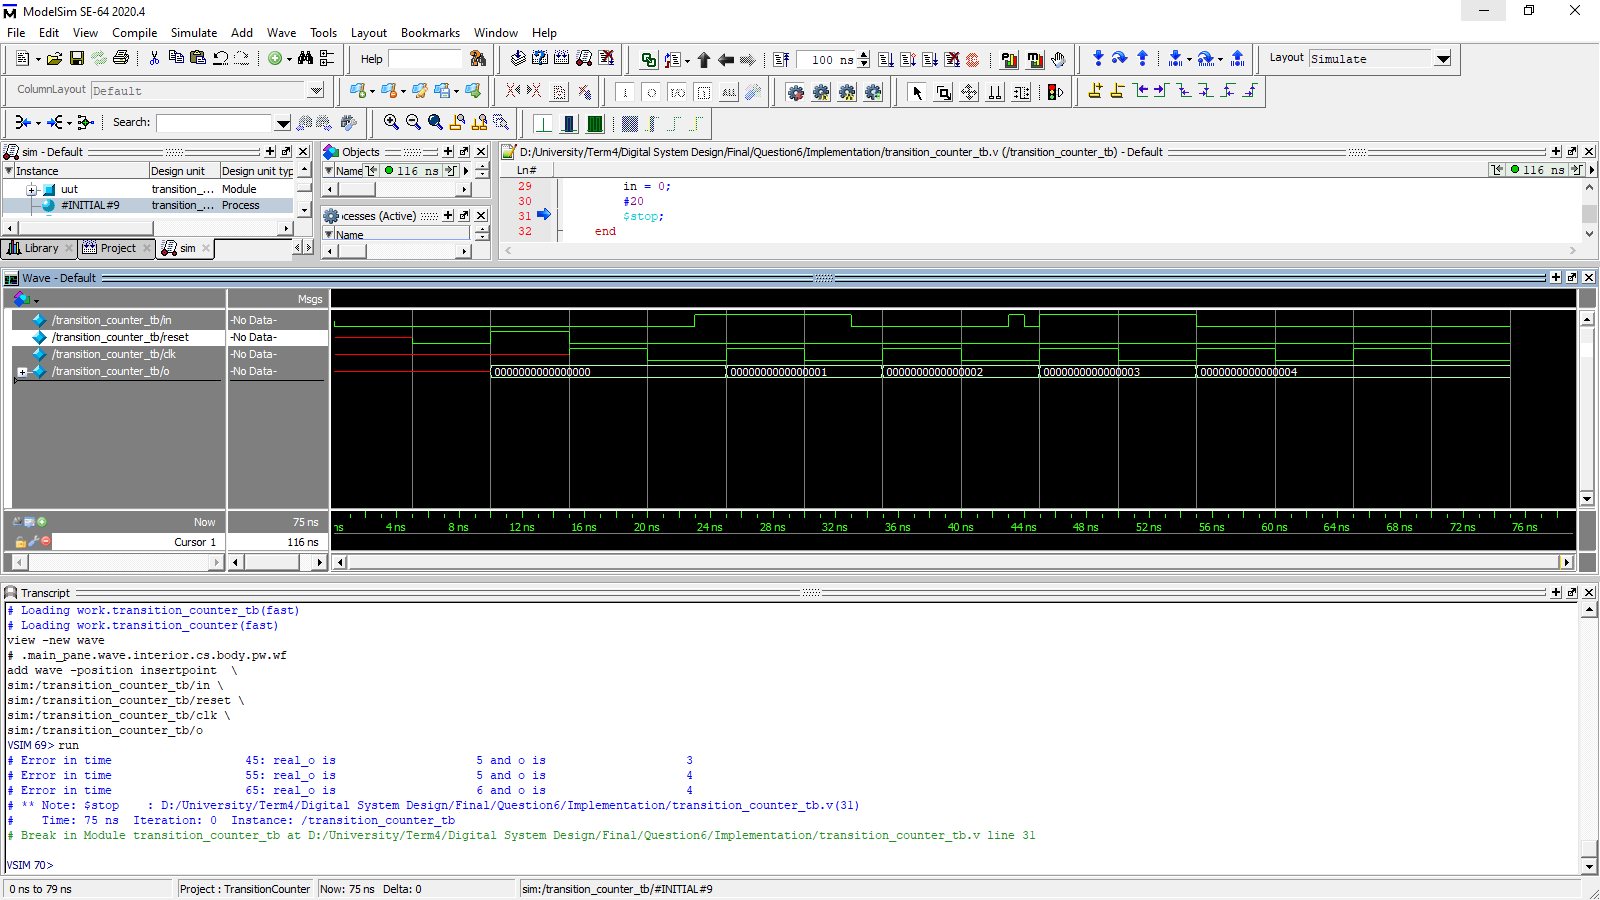
\includegraphics[width=\linewidth]{6.png}
	\caption{نتیجه اجرای شبیه‌سازی \lr{transition counter}}
	\label{simulate6}
\end{figure}

\section{سوال هفت}
\subsection{پیاده‌سازی برنامه پایتون}
برنامه نوشته شده که در فایل 
\lr{dataflow2behavioral/main.py} 
موجود است به صورت 
\begin{latin}
	python main.py -i <inputFile> -o <outputFile>
\end{latin}
اجرا شده و 
\lr{inputFile} 
را مورد پردازش قرار می‌دهد و حاصل را در 
\lr{outputFile}
می‌ریزد.

\subsection{تست کردن برنامه}


\end{document}